\subsection{実験3 ロボットマニピュレータ軌道予測問題における速度変化に対するモデル精度評価}
提案手法をロボットマニピュレータのエンドエフェクタ軌道予測問題に適用し, 軌道速度変化に対するモデル精度評価を行う.

\subsubsection{実験環境}
実験環境は物理シミュレータであるMujoco\cite{mujoco}を用いた.
また, ロボットマニピュレータは6つの自由度を持つUR5eを用いた.
UR5eの構成図とDenavit-Hartenbergパラメータ (DHパラメータ)をそれぞれ\figref{fig:ur5e:structure}と\tabref{tab:ur5e:dh}に示す.
UR5eの制御は目標手先位置から目標関節角度を逆運動学で求め, PD制御によって行った.
ここで, PD制御におけるPゲイン$K_p$, Dゲイン$K_d$はそれぞれ$1$, $0.1$とした.
また, 目標関節角度の計算はMujocoにおける微分運動学ライブラリであるmink\cite{mink}を用いた.
\begin{figure}[htb]
    \centering
    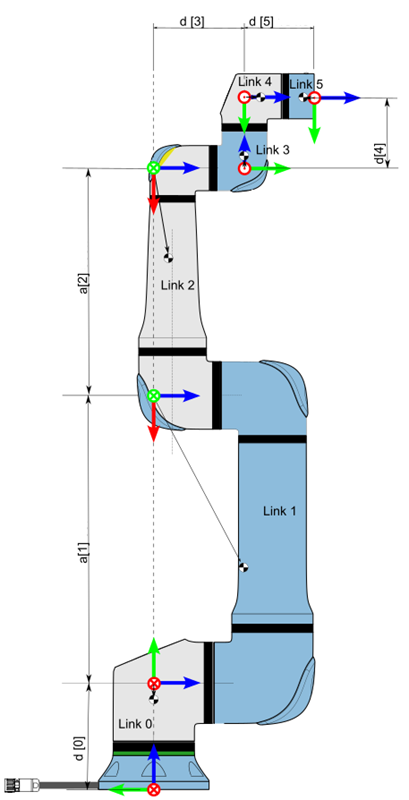
\includegraphics[width=0.5\textwidth]{Static/ur5e_structure.png}
    \caption{UR5eの構成図 \cite{ur5e}}
    \label{fig:ur5e:structure}
\end{figure}

\begin{table}[htb]
    \centering
    \caption{UR5eのDHパラメータ \cite{ur5e}}
    \label{tab:ur5e:dh}
    \begin{tabular}{ccccc}
        \hline
        \textbf{Joint} & $\bm{\theta}$ [rad] & $\bm{a}$ [m]& $\bm{d}$ [m]& $\bm{\theta}$ [rad]\\
        \hline
        1 & 0 & 0       & 0.1625 & $\pi/2$\\
        2 & 0 & -0.425  & 0       & 0\\
        3 & 0 & -0.3922 & 0       & 0\\
        4 & 0 & 0       & 0.1333 & $\pi/2$\\
        5 & 0 & 0       & 0.0997 & $-\pi/2$\\
        6 & 0 & 0       & 0.0996 & 0\\
        \hline
    \end{tabular}
\end{table}


\subsubsection{モデルの学習}
マニピュレータの関節角度の時系列データ$\bm{q}_{t-T \sim t}$を入力, 次の時刻の目標のエンドエフェクタの位置変化量$\bm{dx}_{t}$を出力とするニューラルネットワークを学習する (\eqrefc{eq:model:learning}).
\begin{equation}
    \bm{dx}_{t} = f_{\theta}(\bm{q}_{t-T \sim t}) \label{eq:model:learning}
\end{equation}
ここで, $f_{\theta}$はニューラルネットワーク, $T$は時系列の長さを表す.
目標軌道は$xy$平面における8の字軌道とし, その軌道は\eqrefc{eq:model:target_trajectoryx}, \eqrefc{eq:model:target_trajectoryy}で表される.
\begin{equation}
    x_t=0.25 \sin (\frac{\pi}{5} t) \label{eq:model:target_trajectoryx}
\end{equation}
\begin{equation}
    y_t=0.075 \sin (\frac{2\pi}{5} t) \label{eq:model:target_trajectoryy}
\end{equation}
本実験では1ステップあたりの時間間隔を$0.07$ s, シーケンス全体が$250$ sの軌道を学習に用いた.
また, $z$座標は$z=0.3$ mで固定した.

% 入力
入力であるマニピュレータの関節角度$\bm{q}$は連続値であるため, SNNに入力するために0か1のスパイクに変換する必要がある.
本実験ではスパイク変換のエンコーダとしてThreshold Encodingを用いた.
このエンコーダは, 入力の変化がある閾値$q_{th}$を超えたときに1を出力し, それ以外の場合は0を出力するものである.
ここで, 閾値$q_{th}$を$q_{th}^{max}$から$q_{th}^{min}$までの範囲で$N_{th}$個に分割することで, 入力の変化を$N_{th}$チャンネルのスパイクとして表現することができる.
本実験では入力関節角度は正規化し, $q_{th}^{max}=1.1$, $q_{th}^{min}=-1.1$, $N_{th}=200$とした.

% モデルタイプ
学習させるモデルは通常のSNNおよび提案手法のSNNとした.
それぞれのモデル構成は大きく2つに分けられ, 1つはSNNによる特徴抽出器$f_{\theta}^{SNN}$, もう一つはNNによる予測器$f_{\theta}^{NN}$である.
SNNの出力は0か1のスパイクであるため, 連続値であるエンドエフェクタ座標を直接予測することは困難である.
そこで, 本実験ではSNNを時系列入力の特徴抽出器として扱う.
さらに, SNNの最終層の内部状態$\bm{v}$を特徴量として, 通常のNNで構成された予測器に入力する.
そして, NNによる予測器が教師エンドエフェクタの座標との誤差が小さくなるようにモデルの学習を行う.
ここで, SNNの最終層の内部状態閾値$v_{th}$は無限大とし, 内部状態がリセットされないようにした.
これはSNNのみでVariational Autoencoder (VAE)を構築したFully Spiking VAE (FSVAE)\cite{fsvae}を参考にした構造である.
また, NN予測器の活性化関数はReLU関数とした.
モデルサイズと学習時のパラメータを\tabref{tab:exp3:model:snn} - \tabref{tab:exp3:train:parameter}に示す.
\begin{table}[htb] %\20241112\\eight_figure_shallow3\\snn_beta0.95_seq50",
    \centering
    \caption{マニピュレータ軌道予測モデル : SNN特徴抽出器$f_{\theta}^{SNN}$}
    \label{tab:exp3:model:snn}
    \begin{tabular}{ccc}
        \hline
        \textbf{Input size}& \textbf{Hidden size} & \textbf{Output size}\\
        \hline
        1200   & 512, 256, 128 & 128 \\
        \hline
    \end{tabular}
\end{table}

\begin{table}[htb]
    \centering
    \caption{LIFモデルのパラメータ}
    \label{tab:exp3:model:parameter:lif}
    \begin{tabular}{ccccc}
        \hline
        $\bm{dt}$& $\bm{v_{rest}}$ & $\bm{v_{th}}$ & $\bm{\tau}$ & $\bm{r}$\\
        \hline
        0.03   & 0.0 & 0.1 (最終層のみ$\infty$) & 0.6 & 1 \\
        \hline
    \end{tabular}
\end{table}

\begin{table}[htb] %\20241112\\eight_figure_shallow3\\snn_beta0.95_seq50",
    \centering
    \caption{マニピュレータ軌道予測モデル : NN予測器$f_{\theta}^{NN}$}
    \label{tab:exp3:model:nn}
    \begin{tabular}{ccc}
        \hline
        \textbf{Input size}& \textbf{Hidden size} & \textbf{Output size}\\
        \hline
        128   & 64, 64, 64 & 2 \\
        \hline
    \end{tabular}
\end{table}

\begin{table}[htb]
    \centering
    \caption{モデルの学習条件}
    \label{tab:exp3:train:parameter}
    \begin{tabular}{cc}
        \hline
        学習率 $lr$ & 0.001\\
        バッチサイズ $batch\_size$ & 64\\
        エポック数 $epoches$ & 200\\
        勾配クリッピング $clip\_norm$ & 1.0\\
        optimizer & Adam\\
        \hline
    \end{tabular}
\end{table}

学習時の損失関数を\eqrefc{eq:exp3:loss}に示す.
\begin{align}
    \bm{v}^{t,L} &= f_{\theta}^{SNN}(\bm{q}_{t}) \notag \\
    \bm{\hat{dx}}_{t} &= f_{\theta}^{NN}(\bm{v}^{t,L}) \notag \\
    \mathcal{L_{MSE}} &= \frac{1}{T} \sum_{t=1}^{T} \left( \bm{dx}_{t} - \bm{\hat{dx}}_{t} \right)^2 \label{eq:exp3:loss}
\end{align}
ここで, $\bm{v}^{t,L}$は時刻$t$におけるSNNの最終層の内部状態, $\bm{\hat{dx}}^{t}$は時刻$t$における予測器の出力, $\bm{dx}^{t}$は時刻$t$における目標エンドエフェクタ座標である.
また, 損失関数$L_{MSE}$は入力シーケンスの全ての時刻における予測器の出力と教師データの二乗誤差の平均である.


\subsubsection{評価方法}
学習済みのモデルを用いて, 軌道速度変化に対するモデル精度評価を行う.
軌道速度変化は\eqrefc{eq:exp3:target_trajectoryx}によって行う.
\begin{equation}
    \bm{x}_{t+1}^{target} = \bm{x}_{t} + \frac{\bm{\hat{dx}}_{t}} {a} \label{eq:exp3:target_trajectoryx}
\end{equation}
ここで, $\bm{x}_{t}$は現在のエンドエフェクタの座標, $\bm{\hat{dx}}_{t}$はモデルの出力, $\bm{x}_{t+1}^{target}$は目標のエンドエフェクタ座標である.
また, $a$は軌道速度変化倍率である.
速度倍率$a$は0.1, 0.2, 0.3, 0.4, 0.5, 0.6, 0.7, 0.8, 0.9, 1.0, 2.0, 3.0, 4.0, 5.0とした.
それぞれの速度倍率に対して4周期分の軌道の予測および制御を行い, その軌道と目標軌道のMSEを評価した.

